\chapter{Risk Propagation}\label{ch:risk-propagation}

Risk propagation is a message-passing algorithm that estimates an individual's infection risk by considering their demographics, symptoms, diagnosis, and contact with others. Formally, a \define{risk score} $\vScore_t$ is a timestamped infection probability where $\vScore \in [0, 1]$ and $t \in \naturals$ is the time of its computation. Thus, an individual with a high risk score is likely to test positive for the infection and poses a significant health risk to others. There are two types of risk scores: \define{symptom scores}, or prior infection probabilities, which account for an individual's demographics, symptoms, and diagnosis \citep{Menni2020}; and \define{exposure scores}, or posterior infection probabilities, which incorporate the risk of direct and indirect contact with others.

Given their recent risk scores and contacts, an individual's exposure score is derived by marginalizing over the joint infection probability distribution. Naively computing this marginalization scales exponentially with the number of variables (i.e., individuals). To circumvent this intractability, the joint distribution is modeled as a factor graph, and an efficient message-passing procedure is employed to compute the marginal probabilities with a time complexity that scales linearly in the number of factor nodes (i.e., contacts).

Let $\vGraph = (\vVariables, \vFactors, \vEdges)$ be a \define{factor graph} where $\vVariables$ is the set of variable nodes, $\vFactors$ is the set of factor nodes, and $\vEdges$ is the set of edges incident between them \citep{Kschischang2001}. 

A \define{variable node} $\vVariable: \eventSpace \rightarrow \{0, 1\} $ is a random variable that represents the infection status of an individual, where the sample space is $\eventSpace = \{\var{healthy}, \var{infected}\}$ and
\begin{equation*}
  \vVariable(\event) =
    \begin{cases}
      0 & \text{if } \event = \var{healthy} \\
      1 & \text{if } \event = \var{infected}.
    \end{cases}
\end{equation*}
Thus, $\pr{\vVariable[i]}[t] = \vScore_t$ is a risk score of \indexed{i}{individual}.

A \define{factor node} $\vFactor: \vVariables \times \vVariables \rightarrow [0, 1]$ defines the transmission of infection risk between two contacts. Specifically, contact between \twoindexed{i}{j}{individual} is represented by the factor node $\vFactor(\vVariable[i], \vVariable[j])$ = $\vFactor[ij]$, which is adjacent to the variable nodes $\vVariable[i], \vVariable[j]$. This work and \citet{Ayday2021} assume risk transmission is a symmetric function, $\vFactor[ij] = \vFactor[ji]$. However, it may be extended to account for an individual's susceptibility and transmissibility such that $\vFactor[ij] \neq \vFactor[ji]$. \Cref{fig:factor-graph} depicts a factor graph that reflects the domain constraints.

\begin{figure}[htb]
\centering
\begin{tikzpicture}[ampersand replacement=\&]
  \matrix[row sep=1.5em, column sep=0.75em] {
    \& \factor[minimum size=1em] {f12} {above:$\vFactor[12]$} {} {}; \&\&
    \factor[minimum size=1em] {f23} {above:$\vFactor[23]$} {} {}; \& \\
    \node[latent, minimum size=2em] (v1) {$\vVariable[1]$}; \&\&
    \node[latent, minimum size=2em] (v2) {$\vVariable[2]$}; \&\&
    \node[latent, minimum size=2em] (v3) {$\vVariable[3]$}; \\
  };
  \edge[-] {v1} {f12};
  \edge[-] {v2} {f12};
  \edge[-] {v2} {f23};
  \edge[-] {v3} {f23};
\end{tikzpicture}
\caption[Factor graph]{A factor graph of 3 variable nodes and 2 factor nodes.}
\label{fig:factor-graph}
\end{figure}

\section{Synchronous Risk Propagation}\label{sec:synchronous}

\newcommand{\pDiff}{\epsilon}
\newcommand{\topK}[1]{\text{top } K \text{ of } #1}
\newcommand{\vRiskScores}[2]{\vSet{R}_{#1}^{(#2)}}
\newcommand{\vExposureScore}[2]{r_{#1}^{(#2)}}
\newcommand{\vExposureScores}[1]{\mathbf{r}^{(#1)}}
\newcommand{\dist}{d}

\citet{Ayday2021} first proposed risk propagation as a synchronous, iterative message-passing algorithm that uses the factor graph to compute exposure scores. The first input to \cRiskPropagation{} is the set family $\vScores$, where
\begin{equation} \label{eq:score-set}
  \vScores_i =\setBuilder{\vScore_t}{\vRefTime - t < \pScoreExpiry} \in \vScores
\end{equation}
is the set of recent risk scores of \indexed{i}{individual}. The second input to \cRiskPropagation{} is the contact set
\begin{equation} \label{eq:contact-set}
  \vContacts = \setBuilder{(i, j, t)}{i \neq j, \vRefTime - t < \pContactExpiry}
\end{equation}
such that $(i, j, t)$ is the \emph{most recent} contact between \twoindexed{i}{j}{individual} that occurred from time $t$ until at least time $t + \pMinContactDuration$, where $\pMinContactDuration \in \naturals$ is the \define{minimum contact duration}\footnote{While \citet{Ayday2021} require contact over a $\pMinContactDuration$-contiguous period of time, the Centers for Disease Control and Prevention \citeyearpar{CDC2021} account for contact over a 24-hour period.}. Naturally, risk scores and contacts have finite relevance, so \Cref{eq:score-set} and \Cref{eq:contact-set} are constrained by the \define{risk score expiry} $\pScoreExpiry \in \naturals$ and the \define{contact expiry} $\pContactExpiry \in \naturals$, respectively. The \define{reference time} $\vRefTime \in \naturals$ defines the relevance of the inputs and is assumed to be the time at which \cRiskPropagation{} is invoked. For notational simplicity in \cRiskPropagation{}, let $\vSomeSet$ be a set. Then $\max \vSomeSet = 0$ if $\vSomeSet = \emptyset$.

\subsection{Variable Messages}

The current exposure score of \indexed{i}{individual} is defined as $\max \vScores_i$. Hence, a \define{variable message} $\vVariableMessage{i}{j}{n}$ from the variable node $\vVariable[i]$ to the factor node $\vFactor[ij]$ during \indexed{n}{iteration} is the set of maximal risk scores $\vRiskScores{i}{n - 1}$ from the previous $n - 1$ iterations that were not derived by $\vFactor[ij]$. In this way, risk propagation is reminiscent of the max-sum algorithm; however, risk propagation aims to maximize \emph{individual} marginal probabilities rather than the joint distribution \cite[pp. 411--415]{Bishop2006}.

\subsection{Factor Messages}

A \define{factor message} $\vFactorMessage{i}{j}{n}$ from the factor node $\vFactor[ij]$ to the variable node $\vVariable[j]$ during \indexed{n}{iteration} is an exposure score of \indexed{j}{individual} that is based on interacting with those at most $n - 1$ degrees separated from \indexed{i}{individual}. This population is defined by the subgraph induced in $\vGraph$ by
\begin{equation*}
  \setBuilder{v \in \vVariables \cap \vFactors \setminus \{\vVariable[j], \vFactor[ij]\}}{\dist(\vVariable[i], v) \leq 2(n - 1)},
\end{equation*}
where $\dist(u, v)$ is the distance between the nodes $u, v$. The computation of a factor message assumes the following.
\begin{enumerate}
  \item Contacts have a nondecreasing effect on an individual's exposure score.
  \item A risk score $\vScore_t$ is \define{relevant} to the contact $(i, j, t_{ij})$ if $t < t_{ij} +\pTimeBuffer$, where $\pTimeBuffer \in \naturals$ is a \define{time buffer} that accounts for the incubation period, along with the delayed reporting of symptom scores and contacts. The expression $t_{ij} +\pTimeBuffer$ is called the \define{buffered contact time}.
  \item Risk transmission between contacts is incomplete. Thus, a risk score decays exponentially along its transmission path in $\vGraph$ at a rate of $\log \pTransmissionRate$, where $\pTransmissionRate \in (0, 1)$ is the \define{transmission rate}. \Cref{fig:decay} visualizes this decay, assuming a transmission rate of $\pTransmissionRate = 0.8$ \citep{Hamner2020}.\end{enumerate}

\begin{figure}[htb]
\centering
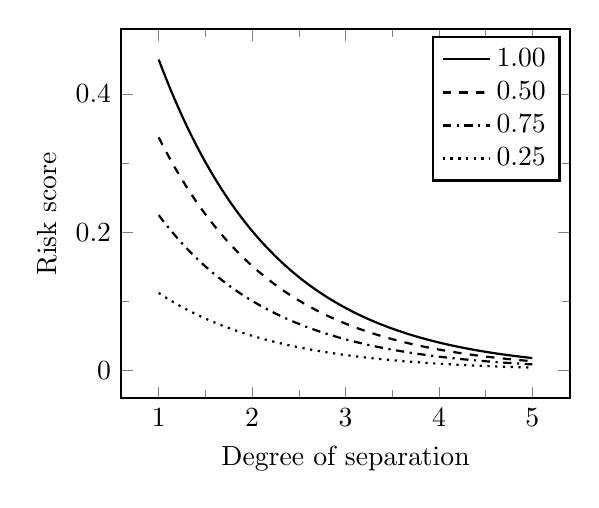
\begin{tikzpicture}
\begin{axis}[
  xlabel={Degree of separation},
  ylabel={Risk score},
  minor tick num=1,
  width=0.6\textwidth,
  smooth,
  domain=1:5,
  y domain=0.01:1,
  samples=100,
  black,
  thick
]
  \addplot[] {e^(-0.8 * x)};
  \addplot[dashed] {0.75 * e^(-0.8 * x)};
  \addplot[dashdotted] {0.5 * e^(-0.8 * x)};
  \addplot[dotted] {0.25 * e^(-0.8 * x)};
  \legend{$1.00$, $0.50$, $0.75$, $0.25$};
\end{axis}
\end{tikzpicture}
\caption[Exponential decay of risk scores]{Exponential decay of risk scores.}
\label{fig:decay}
\end{figure}

To summarize, a factor message $\vFactorMessage{i}{j}{n}$ is the maximum relevant risk score in the variable message $\vVariableMessage{i}{j}{n}$ (or 0) that is scaled by the transmission rate $\pTransmissionRate$.

\citet{Ayday2021} assume that the contact set $\vContacts$ may contain (1) multiple contacts between the same two individuals and (2) \define{invalid} contacts, or those lasting less than $\pMinContactDuration$ time. However, these assumptions introduce unnecessary complexity. Regarding assumption 1, suppose \twoindexed{i}{j}{individual} come into contact $m$ times such that $t_k < t_\ell$ for $1 \leq k < \ell \leq m$. Let $\vFactorMessages_k$ be the set of relevant risk scores, according to the contact time $t_k$, where
\begin{equation*}
  \vFactorMessages_k = \setBuilder{\pTransmissionRate \vScore_t}{\vScore_t \in \vVariableMessage{i}{j}{n}, t < t_k + \pTimeBuffer}.
\end{equation*}
Then $\vFactorMessages_k \subseteq \vFactorMessages_\ell$ if and only if $\max \vFactorMessages_k \leq \max \vFactorMessages_\ell$. Therefore, only the most recent contact time $t_m$ is required to compute the factor message $\vFactorMessage{i}{j}{n}$. With respect to assumption 2, there are two possibilities.
\begin{enumerate}
  \item If an individual has at least one valid contact, then their exposure score is computed over the subgraph induced in $\vGraph$ by their contacts that define the neighborhood $\vNeighbors_i$ of the variable node $\vVariable_i$.
  \item If an individual has no valid contacts, then their exposure score is $\max \vScores_i$ or $0$, if all of their previously computed risk scores have expired.
\end{enumerate}
In either case, a set $\vContacts$ containing only valid contacts implies fewer factor nodes and edges in the factor graph $\vGraph$. Consequently, the complexity of \cRiskPropagation{} is reduced by a constant factor since fewer messages must be computed.

\subsection{Termination}

To detect convergence, the normed difference between the current and previous exposure scores is compared to the threshold $\pDiff \in \reals$. Note that $\vExposureScores{n}$ is the vector of exposure scores in the \indexed{n}{iteration} such that $\vExposureScore{i}{n}$ is \indexed{i}{component} of $\vExposureScores{n}$. The $\ell^1$ and $\ell^\infty$ norms are sensible choices for detecting convergence. \citet{Ayday2021} use the $\ell^1$ norm, which ensures that an individual's exposure score changed by at most $\pDiff$ after the penultimate iteration.

\begin{function}[H]{\nRiskPropagation}[\vScores, \vContacts]
  \State $(\vVariables, \vFactors, \vEdges) \assign \cCreateFactorGraph[\vContacts]$
  \State $n \assign 1$
  \ForEach{$\vVariable[i] \in \vVariables$}
    \State $\vRiskScores{i}{n - 1} \assign \topK{\vScores_i}$
    \State $\vExposureScore{i}{n - 1} \assign \max \vRiskScores{i}{n - 1}$
    \State $\vExposureScore{i}{n} \assign \infty$
  \EndFor
  \While{$\| \vExposureScores{n} - \vExposureScores{n - 1} \| > \pDiff$}
    \ForEach{$\{\vVariable[i], \vFactor[ij]\} \in \vEdges$}
      \State $\vVariableMessage{i}{j}{n} \assign \vRiskScores{i}{n - 1} \setminus \setBuilder{\vFactorMessage{j}{i}{k}}{k \in [1 \twodots n - 1]}$
    \EndFor
    \ForEach{$\{\vVariable[i], \vFactor[ij]\} \in \vEdges$}
      \State $\vFactorMessage{i}{j}{n} \assign \max \setBuilder{\pTransmissionRate \vScore_t}{\vScore_t \in \vVariableMessage{i}{j}{n}, t < t_{ij} + \pTimeBuffer}$
    \EndFor
    \ForEach{$\vVariable[i] \in \vVariables$}
      \State $\vRiskScores{i}{n} \assign \topK{\setBuilder{\vFactorMessage{j}{i}{n}}{\vFactor[ij] \in \vNeighbors_i}}$
    \EndFor
    \ForEach{$\vVariable[i] \in \vVariables$}
      \State $\vExposureScore{i}{n - 1} \assign \vExposureScore{i}{n}$
      \State $\vExposureScore{i}{n} \assign \max \vRiskScores{i}{n}$
    \EndFor
    \State $n \assign n + 1$
  \EndWhile
  \State \Return $\vExposureScores{n}$
\end{function}

\section{Asynchronous Risk Propagation}\label{sec:asynchronous}

While \cRiskPropagation{} offers proof of concept, it is not viable for real-world application. \cRiskPropagation{} is an \define{offline algorithm} \citep{Cormen2022}, because it requires the contact and health information of all individuals as input. As \citet{Ayday2021} note, this centralization of personal data is not privacy-preserving. \cRiskPropagation{} is also inefficient. Most exposure scores are not likely to change across frequent invocations, which implies communication overhead and computational redundancy. To mitigate this inefficiency, \citet{Ayday2020} suggest running \cRiskPropagation{} once or twice per day. Unfortunately, this cadence introduces substantial delay in updating individuals' exposure scores. In the midst of a pandemic, timely information is essential for individual and collective health.

To address the limitations of \cRiskPropagation{}, \citet{Ayday2021} propose decentralizing the factor graph such that the processing entity associated with \indexed{i}{individual} maintains the state of \indexed{i}{variable node} and the neighboring factor nodes. Applying one-mode projection onto the variable nodes \citep{Zhou2007}, \Cref{fig:projected} illustrates how each entity corresponds to a portion of the factor graph. More generally, \citet{Ayday2021} envision risk propagation as a decentralized communication protocol for informing individuals about their infection risk. Such a message-passing protocol naturally aligns with the \define{actor model} which describes concurrent computation as the sending and processing of messages amongst \define{actors} (\Cref{ch:actor-model}). Since communication is asynchronous in the actor model, risk propagation defined in this way is called \define{asynchronous risk propagation}.

\begin{figure}[htb]
\centering
\begin{tikzpicture}[ampersand replacement=\&]
  \matrix[row sep=7em, column sep=2em] {
    \node[latent, minimum size=2em] (v1) {$\vVariable[1]$}; \&\&\&
    \node[latent, minimum size=2em] (v2) {$\vVariable[2]$}; \&\&\&
    \node[latent, minimum size=2em] (v3) {$\vVariable[3]$}; \\
  };
  \factor[minimum size=1em, above= of v1] {f12_1} {above:$\vFactor[12]$} {} {};
  \factor[minimum size=1em, above= of v2, xshift=-3em] {f12_2} {above:$\vFactor[12]$} {} {};
  \factor[minimum size=1em, above= of v2, xshift=3em] {f23_2} {above:$\vFactor[23]$} {} {};
  \factor[minimum size=1em, above= of v3] {f23_3} {above:$\vFactor[23]$} {} {};
  
  \plate{p1} {(v1)(f12_1)(f12_1-caption)} {};
  \plate{p2} {(v2)(f12_2)(f23_2)(f12_2-caption)(f23_2-caption)} {};
  \plate{p3} {(v3)(f23_3)(f23_3-caption)} {};
  
  \edge[-] {v1} {f12_1};
  \edge[-] {v2} {f12_2};
  \edge[-] {v2} {f23_2};
  \edge[-] {v3} {f23_3};
  \edge[-] {p1} {p2};
  \edge[-] {p2} {p3};
\end{tikzpicture}
\caption[One-mode projection of the factor graph]{One-mode projection onto the variable nodes in \Cref{fig:factor-graph}.}
\label{fig:projected}
\end{figure}

\subsection{Actor Behavior}\label{sec:actor-behavior}

An actor in the ShareTrace actor system corresponds to an individual. The \cCreateActor{} operation \citep{Agha1985} initializes an actor $\vActor$ with the following attributes.
\begin{itemize}
  \item $\aActorExposure$: the current exposure score of the individual. This attribute is either a symptom score, a risk score sent by another actor, or the null risk score (see \cNullRiskScore).
  \item $\aActorContacts$: a \define{dictionary} (\Cref{ch:data-structures}) of contacts. In the context of an actor, a contact is a \define{proxy} \citep{Gamma1995} of the actor that represents an individual with which the individual represented by this actor was physically proximal. That is, if \indexed{i}{individual} interacted with \indexed{j}{individual}, then $\aContacts{\vActor_i}$ contains a contact $\vContact$ such that $\aContactKey = \aContactName$ is a name of \indexed{j}{actor} and $\aContactTime$ is the most recent time of contact. This attribute extends the concept of \emph{actor acquaintances} \citep{Hewitt1977a, Hewitt1977b, Agha1985} to be time-varying.
  \item $\aActorScores$: a dictionary of exposure scores such that $\aScoreKey$ for an exposure score $\vScore$ is the time interval during which $\aActorExposure = \vScore$. The null risk score is returned for queries in which the dictionary does not contain a risk score with a key that intersects the given query interval. \Cref{fig:exposure} depicts a hypothetical step function that $\aActorScores$ represents.
\end{itemize}

\begin{function}[H]{\nNullRiskScore}
  \State $\aScoreValue \assign 0$
  \State $\aScoreTime \assign 0$
  \State $\aScoreSender \assign \nil$
  \State \Return $\vScore$
\end{function}

\begin{function}[H]{\nCreateActor}
  \State $\aActorContacts \assign \emptyset$
  \State $\aActorScores \assign \emptyset$
  \State $\aActorExposure \assign \cNullRiskScore$
  \State \Return $\vActor$
\end{function}

\begin{figure}[htb]
\centering
\begin{tikzpicture}
\begin{axis}[
  xlabel={Time},
  ylabel={Exposure score},
  xtick=\empty,
]
  \addplot [const plot mark right] coordinates {
    (0, 0)
    (2, 0)
    (3, 0.3)
    (6, 0.7)
    (9, 0.6)
    (11, 0.9)
    (15, 0.8)
    (17, 0.4)
  };
\end{axis}
\end{tikzpicture}
\caption[Historical exposure scores of an actor]{Hypothetical history of an individual's exposure score.}
\label{fig:exposure}
\end{figure}

% TODO - reference \Cref{sec:system-model}.
%Note that \cCreateActor{} does not specify a name for the actor. This allows the actor to have multiple names and for them to be specified ``out-of-band.''

The interface of an actor is primarily defined by two types of messages: contacts and risk scores. Based on \Cref{sec:synchronous}, let the \define{time to live} (TTL) of a message be the remaining time of its relevance. The reference time $\vRefTime$ is assumed to be the current time.

\begin{function}{\nRiskScoreTtl}[\vScore]
  \State \Return $\pScoreExpiry - (\vRefTime - \aScoreTime)$
\end{function}

\begin{function}{\nContactTtl}[\vContact]
  \State \Return $\pContactExpiry - (\vRefTime - \aContactTime)$
\end{function}

The \cHandleRiskScore{} operation defines how an actor behaves upon receiving a risk score. The key $\aScoreKey$ initially associated with the risk score $\vScore$ is the time interval during which it is relevant. For the dictionary $\aActorScores$, \cMerge{} preserves the mapping invariant defined above such that risk scores are ordered first by value and then by time. Thus, $\aScoreKey \subseteq [\aScoreTime, \aScoreTime + \pScoreExpiry)$ for all exposure scores in $\aActorScores$. The \cUpdateExposureScore{} operation is the online equivalent of updating an individual's exposure score in \cRiskPropagation{}.

\begin{function}[H]{\nHandleRiskScore}[\vActor, \vScore]
  \If{$\cRiskScoreTtl[\vScore] > 0$}
    \State $\aScoreKey \assign [\aScoreTime, \aScoreTime + \pScoreExpiry)$
    \State $\cMerge[\aActorScores, \vScore]$
    \State $\cUpdateExposureScore[\vActor, \vScore]$
    \ForEach{$\vContact \in \aActorContacts$}
      \State $\cApplyRiskScore[\vActor, \vContact, \vScore]$
    \EndFor
  \EndIf
\end{function}

\begin{function}[H]{\nUpdateExposureScore}[\vActor, \vScore]
  \If{$\aActorExposureValue < \aScoreValue$}
    \State $\aActorExposure \assign \vScore$
  \ElsIf{$\cRiskScoreTtl[\aActorExposure] \leq 0$}
    \State $\aActorExposure \assign \cMaximum[\aActorScores]$
  \EndIf
\end{function}

For the moment, assume that \cApplyRiskScore{} is the online equivalent of computing a factor message (see \Cref{sec:synchronous}). Line \ref{step:scale-by-transmission-rate} indicates that a copy $\vNewScore$ of the risk score $\vScore$ is updated using the transmission rate $\pTransmissionRate$. The \cSend{} operation enables actor communication \citep{Agha1985}.

\begin{function}[H]{\nApplyRiskScore}[\vActor, \vContact, \vScore]
  \If{$\aContactTime + \pTimeBuffer > \aScoreTime$}
    \State $\aNewScoreValue \assign \pTransmissionRate \cdot \aScoreValue$ \label{step:scale-by-transmission-rate}
    \State $\cSend[\aContactName, \vNewScore]$
  \EndIf
\end{function}

The problem with \cApplyRiskScore{} is that it causes risk scores to propagate \textit{ad infinitum}. Unlike \cRiskPropagation{}, a global convergence test is not available to terminate message passing, so it is necessary to define a local condition that determines if a risk score should be sent to another actor. Practically, ``self-terminating'' message-passing is necessary for asynchronous risk propagation to be scalable and cost-efficient.

The intent of sending a risk score to an actor is to update its exposure score. According to \cHandleRiskScore{}, it is only necessary to send an actor risk scores with values that exceed its current exposure score. Thus, an actor can associate a \define{send threshold} with a contact such that the target actor only receives risk scores that exceed the threshold. To permit a trade-off between accuracy and efficiency, let the \define{send coefficient} $\pSendCoefficient \in \reals$ be a scaling factor that is applied to a risk score upon setting the send threshold.

\begin{function}{\nSetSendThreshold}[\vContact, \vScore]
  \State $\aNewScoreValue \assign \pSendCoefficient \cdot \aScoreValue$
  \State $\aContactThreshold \assign \vNewScore$
\end{function}

The \cApplyRiskScore{} operation that incorporates the concept of a send threshold  is defined below. Assuming a finite number of actors, a positive send coefficient guarantees that a risk score has finite propagation.

\begin{function}{\nApplyRiskScore}[\vActor, \vContact, \vScore]
  \If{$\aContactThresholdValue < \aScoreValue \AND \aContactTime + \pTimeBuffer > \aScoreTime$}
    \State $\aNewScoreValue \assign \pTransmissionRate \cdot \aScoreValue$
    \State $\cSetSendThreshold[\vContact, \vNewScore]$
    \State $\cSend[\aContactName, \vNewScore]$
  \EndIf
\end{function}

The \cSetSendThreshold{} operation defines \emph{how} the send threshold is updated, but not \emph{when} it should be updated; the \cUpdateSendThreshold{} operation encapsulates the latter. The second predicate on Line \ref{step:should-update-threshold} stems from the fact that the send threshold is a risk score and thus subject to expiry. The first predicate, however, is more subtle and will be revisited shortly. The \cMaximumOlderThan{} operation is the same as \cMaximum{}, with the constraint that the key of the risk score intersects the query interval $(-\infty, \aContactTime + \pTimeBuffer)$. Thus, the returned risk score is always relevant to the contact. Consistent with \cApplyRiskScore{}, the risk score retrieved from $\aActorScores$ is scaled by the transmission rate and set as the new send threshold.

\begin{function}{\nUpdateSendThreshold}[\vActor, \vContact]
  \If{$\aContactThresholdValue > 0 \AND \cRiskScoreTtl[\aContactThreshold] \leq 0$} \label{step:should-update-threshold}
    \State $\vScore \assign \cMaximumOlderThan[\aActorScores, \aContactTime + \pTimeBuffer]$
    \State $\aNewScoreValue \assign \pTransmissionRate \cdot \aScoreValue$
    \State $\cSetSendThreshold[\vContact, \vNewScore]$
  \EndIf
\end{function}

When evaluating Line \ref{step:should-update-threshold} of \cApplyRiskScore{} above, the send threshold should be current. To ensure this is true, the \cUpdateSendThreshold{} operation should be invoked beforehand. Below is a modified description of \cApplyRiskScore{} that integrates \cUpdateSendThreshold{}.

\begin{function}{\nApplyRiskScore}[\vActor, \vContact, \vScore]
  \State $\cUpdateSendThreshold[\vActor, \vContact]$
  \If{$\aContactThresholdValue < \aScoreValue \AND \aContactTime + \pTimeBuffer > \aScoreTime$}
    \State $\aNewScoreValue \assign \pTransmissionRate \cdot \aScoreValue$
    \State $\cSetSendThreshold[\vContact, \vNewScore]$
    \State $\cSend[\aContactName, \vNewScore]$
  \EndIf
\end{function}

Returning to the first predicate on Line \ref{step:should-update-threshold} of \cUpdateSendThreshold{}, the send threshold has a value of 0 when initially assigning the send threshold to be the null risk score; and when no key in $\aActorScores$ intersects the query interval, so the send threshold is again assigned the null risk score. Suppose the first predicate is omitted from Line \ref{step:should-update-threshold}. Given that \cUpdateSendThreshold{} is the first statement in \cApplyRiskScore{}, it is possible that the send threshold is set prior to sending the target actor a relevant risk score. In the worst case, this prevents \emph{all} risk scores from being sent to that actor, and the corresponding individual is inaccurately provided a low risk of infection. For correct message-passing behavior, the send threshold is updated only when its value is nonzero.

The aforementioned refinements to \cApplyRiskScore{} have focused on ensuring that message passing terminates and behaves correctly over time. To conclude the definition of \cApplyRiskScore{}, a message-passing optimization, called \define{sender-side aggregation} \citep{McCune2015}, will be introduced. Over a given period of time, an actor may receive several risk scores that are subsequently sent to multiple contacts. Rather than sending multiple risk scores, it would be more efficient to just send the final risk score. As a heuristic, \cApplyRiskScore{} can be modified so that a contact ``buffers'' a risk score that the target actor should receive.

\begin{function}{\nApplyRiskScore}[\vActor, \vContact, \vScore]
  \State $\cUpdateSendThreshold[\vActor, \vContact]$
  \If{$\aContactThresholdValue < \aScoreValue \AND \aContactTime + \pTimeBuffer > \aScoreTime$}
    \State $\aNewScoreValue \assign \pTransmissionRate \cdot \aScoreValue$
    \State $\cSetSendThreshold[\vContact, \vNewScore]$
    \If{$\aContactName \notEquals \aScoreSender$}
      \State $\aContactBuffered \assign \vNewScore$
    \EndIf
  \EndIf
\end{function}

When the actor receives a periodic \define{flush timeout} message, all contacts are ``flushed'' by sending each buffered risk score to the target actor. For convenience, the \cHandleFlushTimeout{} operation also removes all expired contacts from $\aActorContacts$. 

\begin{function}[H]{\nHandleFlushTimeout}[\vActor]
  \ForEach{$\vContact \in \aActorContacts$}
    \If{$\aContactBuffered \notEquals \nil$}
      \State $\cSend[\aContactName, \aContactBuffered]$
      \State $\aContactBuffered \assign \nil$
    \EndIf
    \If{$\cContactTtl[\vContact] \leq 0$}
      \State $\cDelete[\aActorContacts, \vContact]$
    \EndIf
  \EndFor
\end{function}

The \cHandleContact{} operation concludes this section on actor behavior. Similar to \cHandleRiskScore{}, expired contacts are not processed. The \cMerge{} operation for $\aActorContacts$ differs from its usage with $\aActorScores$. That is, if a contact with the same key already exists, its contact time is updated to that of the newer contact; all other state of the previous contact is maintained. A risk score from $\aActorScores$ is also applied to the contact to ensure that, if the actor receives no other risk score before the contact expires, the target actor is sent at least one relevant risk score.

\begin{function}{\nHandleContact}[\vActor, \vContact]
  \If{$\cContactTtl[c] > 0$}
    \State $\aContactThreshold \assign \cNullRiskScore$
    \State $\aContactBuffered \assign \nil$
    \State $\aContactKey \assign \aContactName$
    \State $\cMerge[\aActorContacts, \vContact]$
    \State $\vScore \assign \cMaximumOlderThan[\aActorScores, \aContactTime + \pTimeBuffer]$
    \State $\cApplyRiskScore[\vActor, \vContact, \vScore]$
  \EndIf
\end{function}

\subsection{Message Reachability}\label{sec:reachability}

The ShareTrace actor system is a \define{contact network}, a type of \define{temporal network} in which nodes represent individuals and edges indicate contact between them. The contact set $\vContacts$ defined in \Cref{eq:contact-set} is known as the \define{contact sequence} representation of a contact network \citep{Holme2012}. For risk propagation, though, the contact time $t$ is more specifically defined to be the most recent (starting) time of contact.

Contact networks are typically used for epidemiological studies in which the focus is on modeling and analyzing the spreading dynamics of the disease \citep{Riolo2001, Danon2011, Lokhov2014, Craft2015, Pastor-Satorras2015, Koher2019, Zino2021}. The ShareTrace actor network, however, models not the spreading of infection, but the spreading of infection \emph{risk}. As noted by \citet{Holme2012}, the transmission graph proposed by \citet{Riolo2001} ``cannot handle edges where one node manages to not catch the disease.'' By framing the spreading as a continuous process, as opposed to a discrete process, the incomplete transmission of infection is possible to model.

A fundamental concept of reachability in temporal networks is the \define{time-respecting path}: a contiguous sequence of contacts with nondecreasing time. Thus, node $v$ is \define{temporally reachable} from node $u$ if there exists a time-respecting path from $u$ to $v$ \citep{Moody2002}. The following quantities are derived from the notion of a time-respecting path and help quantify reachability in a temporal network \citep{Holme2012}.
\begin{itemize}
  \item The \define{influence set} $\vInfluenceSet_v$ of node $v$ is the set of nodes that $v$ can reach by a time-respecting path.
  \item The \define{source set} $\vSourceSet_v$ of node $v$ is the set of nodes that can reach $v$ by a time-respecting path.
  \item The \define{reachability ratio} $\vReachRatio(\vGraph)$ of a temporal network $\vGraph$ is the average cardinality of an influence set.
\end{itemize}

Generally, a message-passing algorithm (e.g., risk propagation) defines a set of constraints that determine when and what messages are sent from one node to another. Even if operating on a temporal network, those constraints may be more or less strict than requiring temporal reachability. As a dynamic process, message passing on a time-varying network requires a more general definition of reachability that accounts for network topology \emph{and} message-passing semantics \citep{Barrat2013}.

Formally, the \emph{message reachability from node $u$ to node $v$} is the number of edges along the shortest path $\vPath$ that satisfy the message-passing constraints,
\begin{equation*}
  \vMessageReachability(u, v) = \sum_{(i, j) \in \vPath} f(u, i, j, v),
\end{equation*}
where
\begin{equation*}
  f(u, i, j, v) = 
    \begin{cases}
      1 & \text{if all constraints are satisfied} \\ 
      0 & \text{otherwise.}
    \end{cases}
\end{equation*}

Node $v$ is \define{message reachable from node $u$} if there exists a shortest path $\vPath$ such that $\vMessageReachability(u, v) = \card{\vPath}$. The \define{message reachability of node $u$} is the maximum message reachability from node $u$:
\begin{equation}\label{eq:vreach}
  \vMessageReachability(u) = \max_{v \in \vVertices} \, \vMessageReachability(u, v).
\end{equation}

Measures of temporal reachability can be extended to message reachability by only considering the message-reachable nodes:
\begin{align*}
  \vInfluenceSet_u &= \setBuilder{v \in \vVertices}{\vMessageReachability(u, v) = \card{\vPath}} \\
  \vSourceSet_v &= \setBuilder{u \in \vVertices}{\vMessageReachability(u, v) = \card{\vPath}} \\
  \vReachRatio(G) &= \sum_{v \in \vVertices} \card{\vInfluenceSet_v} \cdot \card{\vVertices}^{-1}.
\end{align*}

For asynchronous risk propagation, let $\vPath$ is the set of contact edges along the shortest path from actor $u$ to actor $v$ such that the actors are enumerated $1, \ldots, \card{\vPath}$. Then message reachability is defined as
\begin{equation}\label{eq:reach}
  \vMessageReachability(u, v) = \sum_{(i, j) \in \vPath} [\pTransmissionRate^{i} \vScore_u > \pSendCoefficient \pTransmissionRate \vScore_{ij}] \cdot [t_u < t_{ij} + \pTimeBuffer]
\end{equation}
where $[\cdot]$ is the Iverson bracket\footnote{The \define{Iverson bracket} $[x]$ is the indicator function of the set values for which $x$ is true.}.
The value of \Cref{eq:reach} can be found by associating with each symptom score a unique identifier. If each actor maintains a log of the risk scores it receives, then the set of actors that receive the symptom score or a propagated risk score thereof can be identified. This set of actors defines the induced subgraph on which to compute \Cref{eq:reach} using a shortest-path algorithm \citep{Johnson1977}. 

Regarding efficiency, \labelcref{eq:vreach, eq:source-size, eq:influence-size} provide the means to quantify the communication overhead of a given message-passing algorithm on a temporal network. Moreover, because such metrics capture the temporality of message passing, they can better quantify complexity than traditional graph metrics.

By relaxing the constraint \Cref{eq:contact-const}, it is possible to estimate \Cref{eq:reach} with \Cref{eq:value-const}. The \define{estimated message reachability} of node $u$ to node $v$, denoted $\vEstMsgReach(u, v)$, is defined as follows. Based on \Cref{eq:value-const},
\begin{equation*}
  \pTransmissionRate^{\vEstMsgReach(u, v)} \cdot \vScore_u \leq \pSendCoefficient \cdot \vScore_v,
\end{equation*}
where the left-hand side is the value of the propagated symptom score for actor $u$ when $\vEstMsgReach(u, v) = 1$, and the right-hand side is the value required by some message-reachable actor $v$ to propagate the message received by actor $u$ or some intermediate actor. Solving for $\vEstMsgReach(u, v)$,
\begin{equation}\label{eq:estreach}
  \vEstMsgReach(u, v) \leq \begin{cases} 
      0 & \text{if $\vScore_u = 0$} \\
      \card{\vPath} & \text{if $\vScore_v = 0$} \\
      \log_{\pTransmissionRate}\pSendCoefficient + \log_{\pTransmissionRate}\vScore_v - \log_{\pTransmissionRate}\vScore_u & \text{otherwise.}
    \end{cases}
\end{equation}
\Cref{eq:estreach} indicates that a lower send coefficient $\pSendCoefficient$ will generally result in higher message reachability, at the cost of sending possibly ineffective messages (i.e., risk scores that do not update the exposure score of another actor). Equation \Cref{eq:estreach} also quantifies the effect of the transmission rate $\pTransmissionRate$. Unlike the send coefficient, however, the transmission rate is intended to be derived from epidemiology to quantify disease infectivity and should not be optimized to improve performance.

\begin{figure}[htb]
\centering
\begin{tikzpicture}
\begin{semilogyaxis}[
  xlabel={Symptom score},
  ylabel={Send threshold},
  log ticks with fixed point,
  minor tick num=1,
  ytick={0.01, 0.05, 0.1, 0.25, 0.5, 0.75, 1},
  view={0}{90},
  colormap name=black,
  enlargelimits=0.05
]
  \addplot3 [
    contour lua={
      corners,
      levels={1,2,3,4,5,6,7,8,9,10},
      label distance=230pt,
      contour label style={
        inner sep=1pt,
        every node/.style={black, fill=white}
      }
    },
    domain=0.01:1,
    y domain=0.01:1.01,
    samples=100,
  ] {log2(y / x) / log2(0.8)};
\end{semilogyaxis}
\end{tikzpicture}
\caption[Message reachability for risk propagation]{Message reachability for risk propagation. Contour lines are shown for integral reachability values. Given a symptom score, the contour lines indicate the maximum send threshold that permits sending the risk score.}
\label{fig:reach}
\end{figure}

\section{Mobile Crowdsensing}

\define{Mobile crowdsensing} (MCS) is a ``sensing paradigm that empowers ordinary citizens to contribute data sensed or generated from their mobile devices'' that is aggregated  ``in the cloud for crowd intelligence extraction and human-centric service delivery'' \citep{Guo2015}. Over the past decade, substantial research has been conducted on defining and classifying MCS applications \cite[and references therein]{Capponi2019, Guo2015}. While not discussed in previous work \cite{Ayday2020, Ayday2021}, ShareTrace is a MCS application. The following characterization of ShareTrace assumes the four-layered architecture of a MCS application \cite{Capponi2019}, which offers a comprehensive set of classification criteria that To offer a clear comparison, \Cref{tab:classification} follows the same structure as \citet{Capponi2019}. Some aspects of the architecture, namely sampling frequency and sensor activity, are marked according to how ShareTrace is described in previous work, rather than how it would function to optimize for energy efficiency. More detail is provided below in this regard. When classifying ShareTrace as an MCS application, the following description is helpful:
\begin{quote}
  \emph{ShareTrace is a decentralized, delay-tolerant contact-tracing application that estimates infection risk from proximal user interactions and user symptoms.}
\end{quote}

\subsection{Application Layer}

\subsubsection{Application Tasks}

\paragraph{Task Scheduling}

\emph{Proactive scheduling} allows users to decide when and where they contribute sensing data, while \emph{reactive scheduling} requires that ``a user receives a request, and upon acceptance, accomplishes a task'' \cite{Capponi2019}. ShareTrace follows proactive scheduling where the sensing task is to detect proximal interactions with other users. Naturally, the scheduling of this task is at the discretion of the ShareTrace user.

\paragraph{Task Assignment}

\emph{Centralized assignment} assumes that ``a central authority distributes tasks among users.'' Conversely, with \emph{decentralized assignment}, ``each participant becomes an authority and can either perform the task or forward it to other users. This approach is very useful when users are very interested in specific events or activities'' \cite{Capponi2019}. The latter naturally aligns with ShareTrace in which each user is responsible for their own interactions that are both temporally and spatially specific.

\paragraph{Task Execution}

With \emph{single-task execution}, MCS applications assign one type of task to users, while \emph{multi-task execution} assigns  multiple types of tasks \cite{Capponi2019}. ShareTrace only involves the single task of sensing proximal interactions. Alternatively, ShareTrace could be defined more abstractly as sensing infection risk through interactions and user symtpoms. In this case, ShareTrace would follow a multi-tasked execution model, where the task of sensing user symptoms is achieved through user reporting or bodily sensors.

\subsubsection{Application Users}

\paragraph{User Recruitment}

\emph{Volunteer-based recruitment} is when citizens can ``join a sensing campaign for personal interests{\ldots}or willingness to help the community,'' while \emph{incentive-based recruitment} promotes participation and offers control over the recruitment rate{\ldots}These strategies are not mutually exclusive and users can first volunteer and then be rewarded for quality execution of sensing tasks'' \cite{Capponi2019}. ShareTrace assumes volunteer-based recruitment. However, as a decentralized application (dApp) that aligns with the principles of self-sovereignty, an incentive structure that rewards users with verifiable, high-quality data is plausible.

\paragraph{User Selection}

\emph{User-centric selection} is when ``contributions depend only on participants['] willingness to sense and report data to the central collector, which is not responsible for choosing them.'' \emph{Platform-centric selection} is ``when the central authority directly decides data contributors{\ldots}Platform centric decisions are taken according to the utility of data to accomplish the targets of the campaign'' \cite{Capponi2019}. ShareTrace employs user-centric selection, because the purpose of the application is to passively sense the user's interactions and provide them with the knowledge of their infection risk.

\paragraph{User Type}

A \emph{contributor} ``reports data to the MCS platform with no interest in the results of the sensing campaign'' and ``are typically driven by incentives or by the desire to help the scientific or civil communities.'' A \emph{consumer} joins ``a service to obtain information about certain application scenario[s] and have a direct interest in the results of the sensing campaign'' \cite{Capponi2019}. For ShareTrace, users can be either a consumer or a contributor but are likely biased toward the former.

\subsection{Data Layer}

\subsubsection{Data Management}

\paragraph{Data Storage}

\emph{Centralized storage} involves data being ``stored and maintained in a single location, which is usually a database made available in the cloud. This approach is typically employed when significant processing or data aggregation is required.'' \emph{Distributed storage} ``is typically employed for delay-tolerant applications, i.e., when users are allowed to deliver data with a delayed reporting'' \cite{Capponi2019}. For sensing human interaction, ShareTrace relies on distributed storage in the form of Dataswift Personal Data Accounts. Moreover, ShareTrace is delay-tolerant, so distributed storage is most appropriate. However, for reporting the population-level risk distribution, it is likely that centralized storage would be used.

\paragraph{Data Format}

\emph{Structured data} is standardized and readily analyzable. \emph{Unstructured data}, however, requires significant processing before it can be used \cite{Capponi2019}. ShareTrace deals with structured data (e.g., user symptoms, actor URIs).

\paragraph{Data Dimensionality}

\emph{Single-dimension data} typically occurs when a single sensor is used, while \emph{multi-dimensional data} arises with the use of multiple sensors. ShareTrace data is one-dimensional because it only uses Bluetooth to sense nearby users.

\subsubsection{Data Processing}

\paragraph{Data Pre-processing}

\emph{Raw data output} implies that no modification is made to the sensed data. \emph{Filtering and denoising} entail ``removing irrelevant and redundant data. In addition, they help to aggregate and make sense of data while reducing at the same time the volume to be stored'' \cite{Capponi2019}. ShareTrace only retains the actor URIs that correspond to valid contacts (i.e., lasting at least 15 minutes).

\paragraph{Data Analytics}

\emph{Machine learning} (ML) \emph{and data mining analytics} are not real-time. They ``aim to infer information, identify patterns, or predict future trends.'' On the contrary, \emph{real-time analytics} consist of ``examining collected data as soon as it is produced by the contributors'' \cite{Capponi2019}. ShareTrace aligns with the former category since it aims to infer the infection risk of users.

\paragraph{Data Post-processing}

\emph{Statistical post-processing} ``aims at inferring proportions given quantitative examples of the input data. \emph{Prediction post-processing} aims to determine ``future outcomes from a set of possibilities when given new input in the system'' \cite{Capponi2019}. ShareTrace applies predictive post-processing via risk propagation.

\subsection{Communication Layer}

\subsubsection{Communication Technology}

\paragraph{Infrastructured Technology}

\emph{Cellular} connectivity ``is typically required from sensing campaign[s] that perform real-time monitoring and require data reception as soon as it is sensed.'' \emph{WLAN} ``is used mainly when sensing organizers do not specify any preferred reporting technologies or when the application domain permits to send data'' at ``a certain amount of time after the sensing process'' \cite{Capponi2019}. Infrastructured technology is also referred to as the \emph{infrastructured transmission paradigm} \cite{Ma2014}. ShareTrace does not require cellular infrastructure, because it is delay-tolerant and thus only requires WLAN.

\paragraph{Infrastructure-less Technology}

\emph{Infrastructure-less technologies} ``consists of device-to-device (D2D) communications that do not require any infrastructure{\ldots}but rather allow devices in the vicinity to communicate directly.'' Technologies include \emph{WiFi-Direct}, \emph{LTE-Direct}, and \emph{Bluetooth} \citep{Capponi2019}. Infrastructure-less technology is also called the \emph{opportunistic transmission paradigm} \citep{Ma2014}. ShareTrace uses Bluetooth because of its energy efficiency and short range.

\subsubsection{Data Reporting}

\paragraph{Upload mode}

With \emph{relay uploading}, ``data is delivered as soon as collected.'' \emph{Store-and-forward} ``is typically used in delay-tolerant applications when campaigns do not need to receive data in real-time'' \citep{Capponi2019}. Because ShareTrace is delay-tolerant, it uses store-and-forward uploading.

\paragraph{Metholodgy}

\emph{Individualized sensing} is ``when each user accomplishes the requested task individually and without interaction with other participants.'' \emph{Collaborative sensing} is when ``users communicate with each other, exchange data[,] and help themselves in accomplishing a task or delivering information to the central collector. Users are typically grouped and exchange data exploiting short-range communication technologies, such as WiFi-[D]irect or Bluetooth{\ldots}Note that systems that create maps merging data from different users are considered individual because users do not interact between each other to contribute'' \citep{Capponi2019}. The methodology of sensing is similar to the \emph{sensing scale} which is typically dichotomized as \emph{personal} \citep{Lane2010, Ganti2011} (i.e., individualized) and \emph{community} \citep{Ganti2011} or \emph{group} \citep{Lane2010} (i.e., collaborative). ShareTrace is inherently collaborative, relying on mobile devices to exchange actor URIs to estimate infection risk. Thus, collaborative sensing is used.

\paragraph{Timing}

\emph{Timing} is based on whether devices ``should sense in the same period or not.'' \emph{Synchronous timing} ``includes cases in which users start and accomplish at the same time the sensing task. For synchronization purposes, participants communicate with each other.'' \emph{Asynchronous timing} occurs ``when users perform sensing activity not in time synchronization with other users'' \citep{Capponi2019}. ShareTrace requires synchronous timing, because contact sensing inherently requires synchronous communication between the involved devices.

\subsection{Sensing Layer}

\subsubsection{Sensing Elements}

\paragraph{Sensor Deployment}

\emph{Dedicated deployment} involves the use of ``non-embedded sensing elements,'' typically for a specific task. \emph{Non-dedicated deployment} utilizes sensors that ``do not require to be paired with other devices for data delivery but exploit the communication capabilities of mobile devices'' \citep{Capponi2019}. ShareTrace relies on non-dedicated deployment since it relies on Bluetooth that is ubiquitous in modern-day mobile devices.

\paragraph{Sensor Activity}

\emph{Always-on sensors} ``are required to accomplish mobile devices['] basic functionalities, such as detection of rotation and acceleration{\ldots} Activity recognition [i.e., context awareness]{\ldots}is a very important feature that accelerometers enable.'' \emph{On-demand sensors} ``need to be switched on by users or exploiting an application running in the background. Typically, they serve more complex applications than always-on sensors and consume a higher amount fo energy'' \citep{Capponi2019}. ShareTrace uses Bluetooth, which may be considered on-demand. While energy efficient, users do control when it is enabled. Ideally, ShareTrace would also use always-on sensors to enable Bluetooth with context awareness (i.e., that the user is carrying or nearby the device).

\paragraph{Acquisition}

\emph{Homogeneous acquisition} ``involves only one type of data and it does not change from one user to another one,'' while \emph{heterogeneous acquisition} ``involves different data types usually sampled from several sensors'' \citep{Capponi2019}. ShareTrace is homogeneous, because all users sense the same data from one type of sensor.

\subsubsection{Data Sampling}

\paragraph{Sampling Frequency}

\emph{Continuous sensing} ``indicates tasks that are accomplished regularly and independently [of] the context of the smartphone or the user['s] activities.'' \emph{Event-based sensing} is ``data collection [that] starts after a certain event has occurred. In this context, an event can be seen as an active action from a user or the central collector, but also a given context awareness'' \citep{Capponi2019}. ShareTrace sensing is continuous but would ideally be event-based to conserve device energy.

\paragraph{Sensing Responsibility}

When the \emph{mobile device} is responsible, ``devices or users take sampling decisions locally and independently from the central authority{\ldots}When devices take sampling decisions, it is often necessary to detect the context [of the] smartphones and wearable devices{\ldots}The objective is to maximize the utility of data collection and minimize the cost of performing unnecessary operations.'' When the \emph{central collector} is responsible, they make ``decisions about sensing and communicate them to the mobile devices'' \citep{Capponi2019}. Given the human-centric nature of the ShareTrace sensing task, mobile devices are responsible.

\paragraph{User involvement}

\emph{Participatory involvement} ``requires active actions from users, who are explicitly asked to perform specific tasks. They are responsible to consciously meet the application requests by deciding when, what, where, and how to perform sensing tasks.'' \emph{Opportunistic involvement} means that ``users do not have direct involvement, but only declare their interest in joining a campaign and providing their sensors as a service. Upon a simple handshake mechanism between the user and the MCS platform, a MCS thread is generated on the mobile device (e.g., in the form of a mobile app), and the decisions of what, where, when, and how to perform the sensing are delegated to the corresponding thread. After having accepted the sensing process, the user is totally unconscious with no tasks to perform and data collection is fully automated{\ldots}The smartphone itself is context-aware and makes decisions to sense and store data, automatically determining when its context matches the requirements of an application. Therefore, coupling opportunistic MCS systems with context-awareness is a crucial requirement'' \citep{Capponi2019}. Earlier works on MCS refer to user involvement as the \emph{sensing paradigm} \citep{Lane2010, Ganti2011, Ma2014}. ShareTrace is opportunistic, ideally with context-awareness.

\begin{table}[htb]
\renewcommand{\arraystretch}{0.85}
\scriptsize
\centering
\begin{tabularx}{\textwidth}{
    >{\centering\arraybackslash}X
    >{\centering\arraybackslash}X
    >{\centering\arraybackslash}X
    c
    >{\centering\arraybackslash}X}
\toprule
\multirow{12}*{Application}
	& \multirow{6}*{Task}
		& \multirow{2}*{Scheduling}
			& Proactive & $\bullet$ \\
			&&& Reactive & \\
		\cmidrule{3-5}
		&& \multirow{2}*{Assignment}
			& Centralized & \\
			&&& Decentralized & $\bullet$ \\
		\cmidrule{3-5}
		&& \multirow{2}*{Execution}
			& Single task & $\bullet$ \\
			&&& Multi-tasking & \\
	\cmidrule{2-5}
	& \multirow{6}*{User}
		& \multirow{2}*{Recruitment}
			& Voluntary & $\bullet$ \\
			&&& Incentivized & \\
		\cmidrule{3-5}
		&& \multirow{2}*{Selection}
			& Platform-centric & \\
			&&& User-centric & $\bullet$ \\
		\cmidrule{3-5}
		&& \multirow{2}*{Type}
			& Consumer & $\bullet$ \\
			&&& Contributor & $\bullet$ \\
		\cmidrule{2-5}
\cmidrule{1-5}
\multirow{12}*{Data}
	& \multirow{6}*{Management}
		& \multirow{2}*{Storage}
			& Centralized & \\
			&&& Distributed & $\bullet$ \\
		\cmidrule{3-5}
		&& \multirow{2}*{Format}
			& Structured & $\bullet$ \\
			&&& Unstructured & \\
		\cmidrule{3-5}
		&& \multirow{2}*{Dimension}
			& Single dimension & $\bullet$ \\
			&&& Multi-dimensional & \\
	\cmidrule{2-5}
	& \multirow{6}*{Processing}
		& \multirow{2}*{Pre-processing}
			& Raw data & \\
			&&& Filtering and denoising & $\bullet$ \\
		\cmidrule{3-5}
		&& \multirow{2}*{Analytics}
			& ML and data mining & $\bullet$ \\
			&&& Real-time & \\
		\cmidrule{3-5}
		&& \multirow{2}*{Post-processing}
			& Statistical & \\
			&&& Prediction & $\bullet$ \\
		\cmidrule{2-5}
\cmidrule{1-5}
\multirow{11}*{Communication}
	& \multirow{5}*{Technologies}
		& \multirow{2}*{Infrastructured}
			& Cellular & $\bullet$ \\
			&&& WLAN & $\bullet$ \\
		\cmidrule{3-5}
		&& \multirow{3}*{Infrastructure-less}
			& LTE-Direct & \\
			&&& WiFi-Direct & \\
			&&& Bluetooth & $\bullet$ \\
		\cmidrule{3-5}
	\cmidrule{2-5}
	& \multirow{6}*{Reporting}
		& \multirow{2}*{Upload mode}
			& Relay & \\
			&&& Store and forward & $\bullet$ \\
		\cmidrule{3-5}
		&& \multirow{2}*{Methodology}
			& Individual & \\
			&&& Collaborative & $\bullet$ \\
		\cmidrule{3-5}
		&& \multirow{2}*{Timing}
			& Synchronous & $\bullet$ \\
			&&& Asynchronous & \\
		\cmidrule{2-5}
\cmidrule{1-5}
\multirow{12}*{Sensing}
	& \multirow{6}*{Elements}
		& \multirow{2}*{Deployment}
			& Dedicated & \\
			&&& Non-dedicated & $\bullet$ \\
		\cmidrule{3-5}
		&& \multirow{2}*{Activity}
			& Always-on & $\bullet$ \\
			&&& On-demand & $\circ$ \\
		\cmidrule{3-5}
		&& \multirow{2}*{Acquisition}
			& Homogeneous & $\bullet$ \\
			&&& Heterogeneous & \\
	\cmidrule{2-5}
	& \multirow{6}*{Sampling}
		& \multirow{2}*{Frequency}
			& Continuous & $\bullet$ \\
			&&& Event-based & $\circ$ \\
		\cmidrule{3-5}
		&& \multirow{2}*{Responsibility}
			& Mobile device & $\bullet$ \\
			&&& Central collector & \\
		\cmidrule{3-5}
        && \multirow{2}*{User involvement}
			& Participatory & \\
			&&& Opportunistic & $\bullet$ \\
\bottomrule
\end{tabularx}
\caption[ShareTrace classification]{ShareTrace classification using the four-layered architecture of a mobile crowdsensing application \citep{Capponi2019}. Always ($\bullet$); with context-awareness ($\circ$).}
\label{tab:classification}
\end{table}

\section{System Model}\label{sec:system-model}

% TODO - security and privacy (e.g., PDAs vs local computation)

The system model is similar to that in previous work \citep{Ayday2020, Ayday2021}. \Cref{fig:actor-dataflow} illustrates the corresponding data flow\footnote{A \emph{data-flow diagram} consists of data processors (circles), directed data flow (arrows), data stores (parallel lines), and external entities (rectangles) \cite[pp. 437--438]{Fowler2004}\label{foot:dataflow}.}.
\begin{itemize}
  \item Each user owns a \emph{personal data store} (PDS), a form of cloud storage that empowers the user with ownership and access control over their data.
  \item Symptom scores are computed in a user's PDS to support integrating multiple streams of personal data \citep{Ayday2020}. While local symptom-score computation \citep{Ayday2020, Ayday2021} is more privacy-preserving, it is assumed that the user's PDS is a trusted entity.
  \item User device interactions serve as a proxy for proximal human interactions. This work does not assume a specific protocol, but does assume that the protocol can approximate the duration of contact with relative accuracy and that communication with the actors of those contacted users can be established in a privacy-preserving manner.
  \item No geolocation data is collected \citep{Ayday2020}. As a decentralized, proximity-based solution, it is not necessary to collect user geolocation data. See \Cref{sec:location-based} for a discussion of a geolocation-based design that was considered.
\end{itemize}

\begin{figure}[htb]
    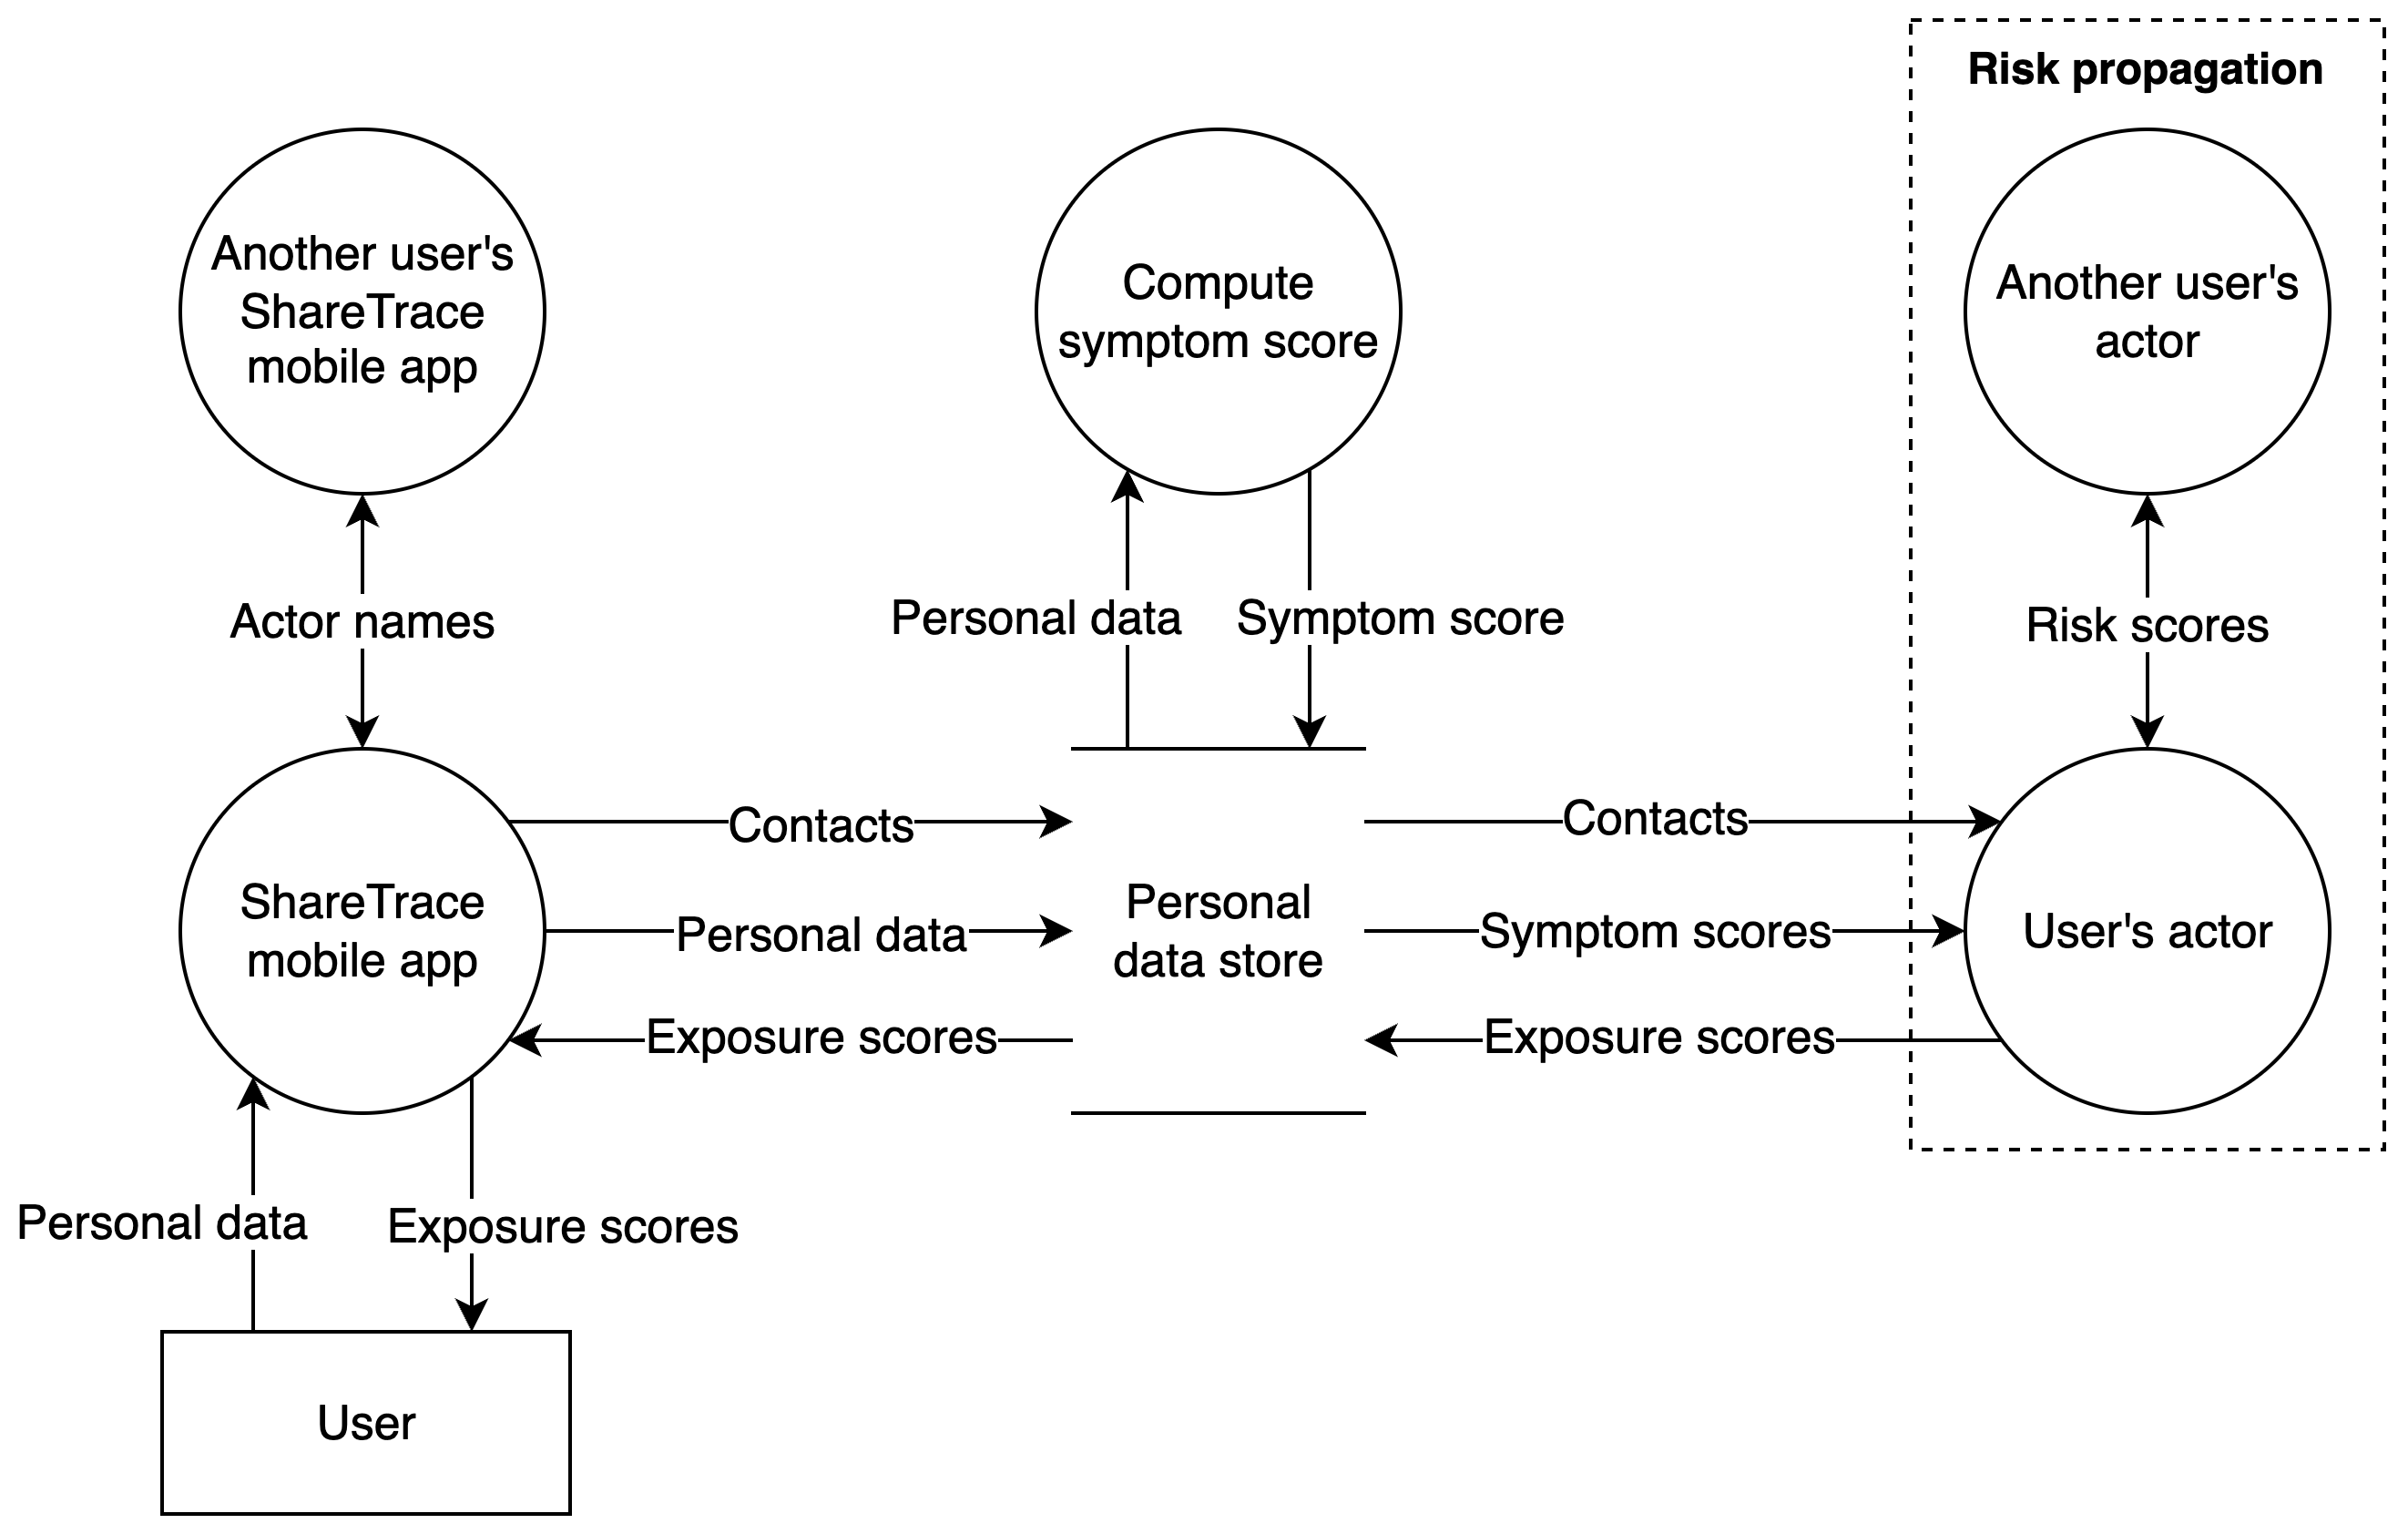
\includegraphics[width=\textwidth]{distributed-dataflow}
    \caption[Distributed ShareTrace data flow]{Distributed ShareTrace data flow. \emph{Contacts} include the actor name and contact time of all users with which the user came into close proximity. \emph{Personal data} includes the user's demographics, reported symptoms, and diagnosis. It may also include machine-generated biomarkers and electronic health record data \citep{Ayday2020}.}
    \label{fig:distributed-dataflow}
\end{figure}

\begin{figure}[htb]
    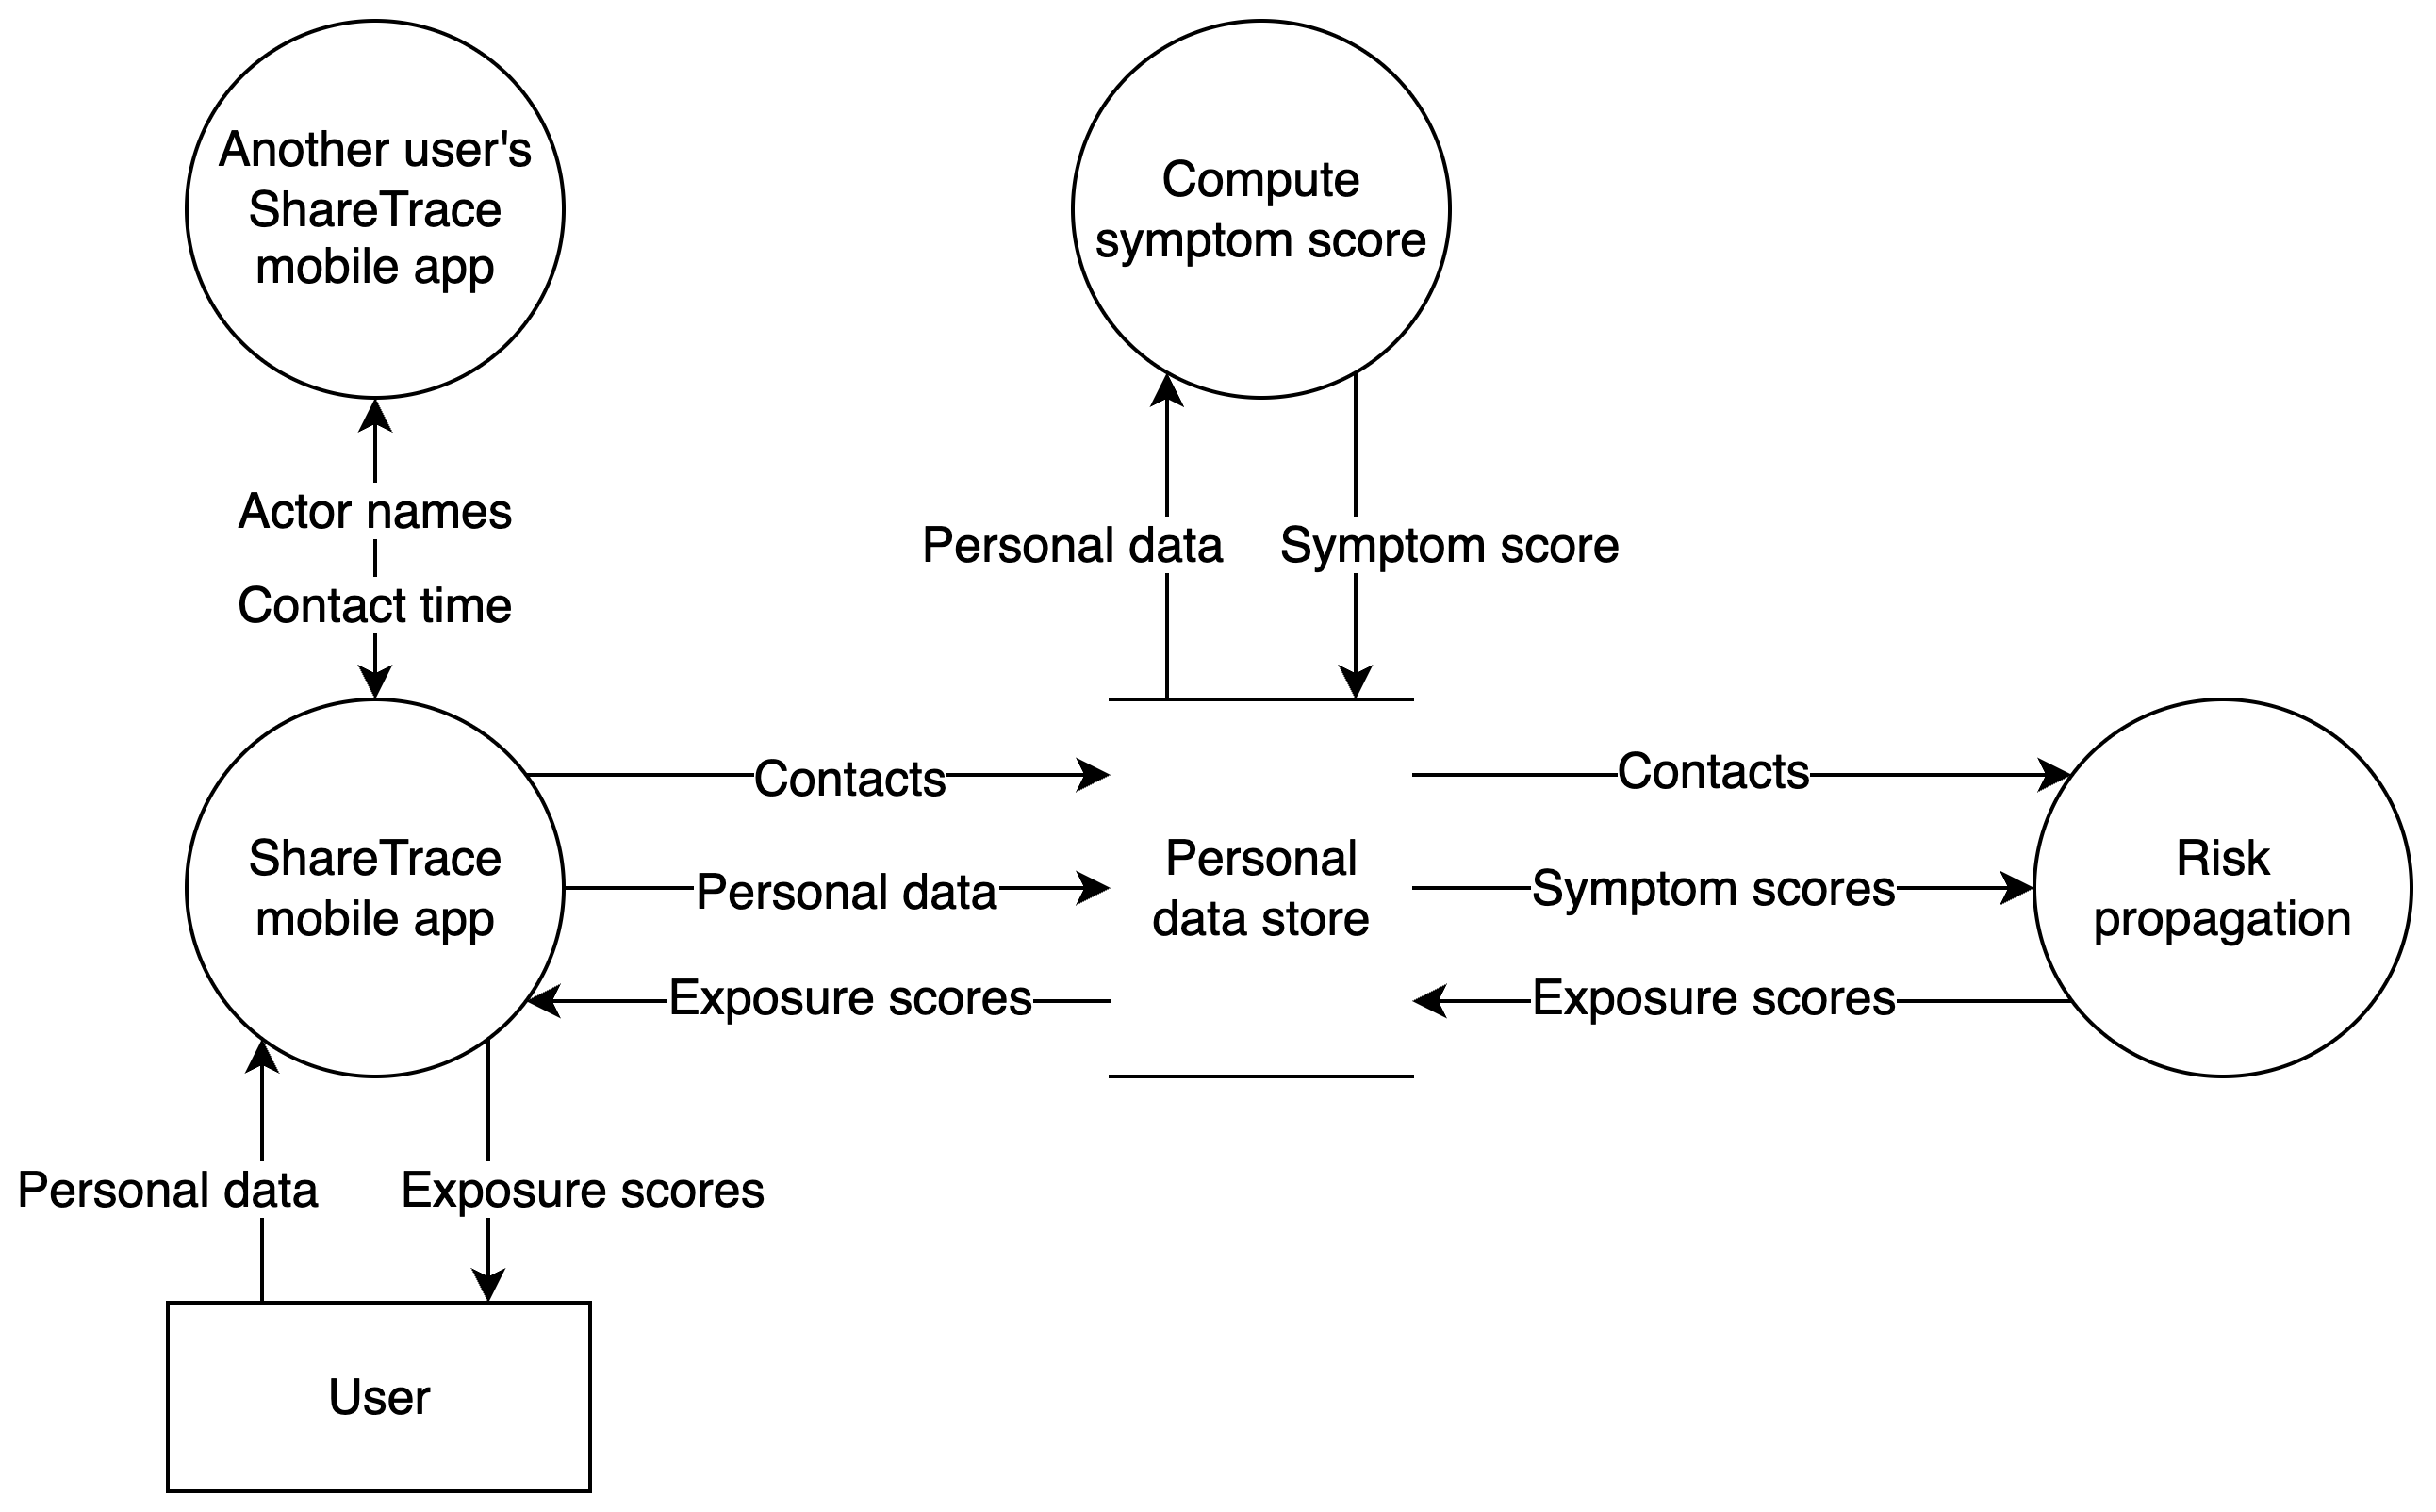
\includegraphics[width=\textwidth]{centralized-dataflow}
    \caption[Centralized ShareTrace data flow]{Centralized ShareTrace data flow. \emph{Contacts} include the actor name and contact timestamp of all users with which the user came into close proximity. \emph{Personal data} includes the user's demographics, reported symptoms, and diagnosis. It may also include machine-generated biomarkers and electronic health record data \citep{Ayday2020}.}
    \label{fig:centralized-dataflow}
\end{figure}